%
% File nodalida2017.tex
%
% Contact beata.megyesi@lingfil.uu.se
%
% Based on the instruction file for Nodalida 2015 and EACL 2014
% which in turn was based on the instruction files for previous 
% ACL and EACL conferences.

\documentclass[11pt]{article}
\usepackage{nodalida2017}
%\usepackage{times}
\usepackage{mathptmx}
%\usepackage{txfonts}
\usepackage{xcolor}
\usepackage{graphicx}
\usepackage{url}
\usepackage{latexsym}
\special{papersize=210mm,297mm} % to avoid having to use "-t a4" with dvips 
%\setlength\titlebox{6.5cm}  % You can expand the title box if you really have to

\title{Exploring the Expressivity of Constraint Grammar}

% \author{First Author \\
%   Affiliation / Address line 1 \\
%   Affiliation / Address line 2 \\
%   Affiliation / Address line 3 \\
%   {\tt email@domain} \\\And
%   Second Author \\
%   Affiliation / Address line 1 \\
%   Affiliation / Address line 2 \\
%   Affiliation / Address line 3 \\
%   {\tt email@domain} \\}

\date{}

\def\t#1{\texttt{#1}}

\def\maxAmb#1{$\langle \Sigma \rangle_#1$}

\def\maxAmbFSA#1{$\langle \Sigma,S \rangle_#1$}

\begin{document}
\maketitle

% \begin{abstract}
%   This document contains the instructions for preparing a camera-ready
%   manuscript for the proceedings of Nodalida-2017. The document itself
%   conforms to its own specifications, and is therefore an example of
%   what your manuscript should look like. These instructions should be
%   used for both papers submitted for review and for final versions of
%   accepted papers.  Authors are asked to conform to all the directions
%   reported in this document.
% \end{abstract}


\section{Introduction}

Traditionally, CG is seen as a practical and language-oriented approach to NLP;
it is a tool rather than a formalism, framework or anything of the sort.
%%% WEN: What's the purpose of this sentence?
Since the beginning of CG~\cite{karlsson1995constraint}, its authors do not
see it as a tool for generating strings, only for analysing and disambiguating
them.
%%% WEN: Well, I'm giving the sentence above purpose here:
It is for these reasons, we believe, that the question of the expressivity of CG
as a generative formalism went unasked and unanswered for so long.
%%% WEN: ^Is this actually true? Or have folks looked into this before?^

We believe that for any formalism which has its roots in linguistics, it is a
natural question to ask ``how expressive is it?''
Therefore, in this paper, we begin to address the question of the expressivity
of CG. 
%%% WEN: We are OBLIGED to make the point here---or at very least NOT too far
%%%      into the paper---that this question has an obvious answer. There is a
%%%      command that allows you to call an arbitrary process, so it is
%%%      obviously Turing complete. However, what we are interested in is how
%%%      expressive the separate COMMANDS in CG are. What can we do with just
%%%      REMOVE---the most common CG command? What can we do if we allow
%%%      ourselves the use of REMOVE and some other command? Etc.
%%% WEN: I'd say it's interesting to look at the formal language aspects BECAUSE
%%%      it's a linguistic tool and therefore comes from a tradition of formal
%%%      language.
% Despite its decidedly linguistic roots, we argue that CG is interesting to look
% at also from a computational perspective.
%%% WEN: So basically you're saying ``we decided to have an academic wank'' it
%%%      was definitely great. ^^
For those theoretically inclined, describing the expressivity of a new language
formalism might be a reward onto itself. 
%%% WEN: This is, like, a super weak claim. xD
However, even the more practical reader could appreciate that a better
understanding of a formalism can lead to novel uses and implementation
techniques. 
%%% WEN: Maybe we could take some of these hopes expressed in the following
%%%      sentence, and rephrase them as novel uses and implementation techniques
%%%      to satisfy our more practical readers? For instance, we could hint at a
%%%      future version of your CGexp library which could be used to
%%%      automatically generate CG code which disambiguates based on some
%%%      regular expressions? You may be the better person to phrase this
%%%      though. But I'll have a go.
For instance, we hope that the \texttt{cgexp} tool, described in later sections
of this paper, could eventually be developed to generate human-readable CG code
which attempts to disambiguate pharses based on regular expressions or a
context-free grammar. 
% ... hope to create new ways to reason about reductionistic grammar formalisms. 


\section{Background and previous work}


The standard measure of formal languages is the Chomsky hierarchy~\cite{chomsky1956hierarchy}, with its four
classes of grammars and languages, in order from most expressive to least expressive:
recursively enumerable (Type 0), context-sensitive (Type 1), context-free (Type 2), and
regular (Type 3).
The notion of expressive power, ``which constructs can we express in the language'', is coupled with parsing complexity, ``how much time and memory do we need to parse sentences in the language''; more expressive power corresponds to greater parsing complexity.

Previous work covers the expressivity of single rules, such as \texttt{IF (NOT 1* Verb OR Noun)}: just seeing this contextual test hints that we can express a subset of regular languages that contains at least disjunction, complement and Kleene star. 
\newcite{tapanainen1999phd} gives a precise definition of the expressivity of a single rule for 4 different constraint formalisms. In addition, parsing complexity can be easily defined for a given variant and implementation of CG; see for instance \newcite{nemeskey14}.

However, the expressivity of the whole grammar is harder to define. 
A given grammar in CG does not describe a language, but a \emph{relation} between an input language and an output language. 
In the following section, we introduce our approach to emulating generation, and in the rest of the paper, we present some preliminary results.

\section{Expressivity of a grammar}

We view a constraint grammar as a formal language $\mathcal{L}$, generated over an 
alphabet $\Sigma$. We generate the strings in our language by passing 
\emph{maximally ambiguous strings} of every length to the grammar. 
With maximally ambiguous, we mean those strings where each cohort contains the 
entire alphabet, written as \maxAmb{n}. 
A constraint grammar is said to accept a string $w$ of length $n$ if, 
when we pass \maxAmb{n} as an input to the CG,
$w$ is one of the possible interpretations of its output.

For example, consider the language $a*$ over $\Sigma = \{a,b\}$,
shown in Figure~\ref{fig:astar}.
%The initial sentence consists of cohorts with two readings, $a$ and $b$, and the disambiguated sentence has only cohorts with a single reading, $a$. 
The grammar that accepts this language is simply \texttt{SELECT (a)}.

\def\wwf{\t{"<w>"}}
\def\swf{\t{"<s>"}}
\def\alm{\t{"a" a}~~~~~~}
\def\blm{\t{"b" b}~~~~~~}

\begin{figure}[h]
\centering

%\begin{tabular}{cl @{\hspace{2cm}} rl}
\begin{tabular}{cl |  rl}
\multicolumn{2}{c|}{\textbf{Input}} & \multicolumn{2}{c}{\textbf{Output}} \\ \hline

\wwf  &        &  \wwf &        \\
         & \alm  &          & \alm  \\
         & \blm  &          &        \\
\wwf  &        &  \wwf &        \\
         & \alm  &          & \alm  \\
         & \blm  &          &        \\
\wwf  &        &  \wwf &        \\
         & \alm  &          & \alm  \\
         & \blm  &          &        \\
\end{tabular}

\caption{Language $a*$ for input \maxAmb{3}.}
\label{fig:astar}
\end{figure}



\begin{figure}[t]
  \centering
    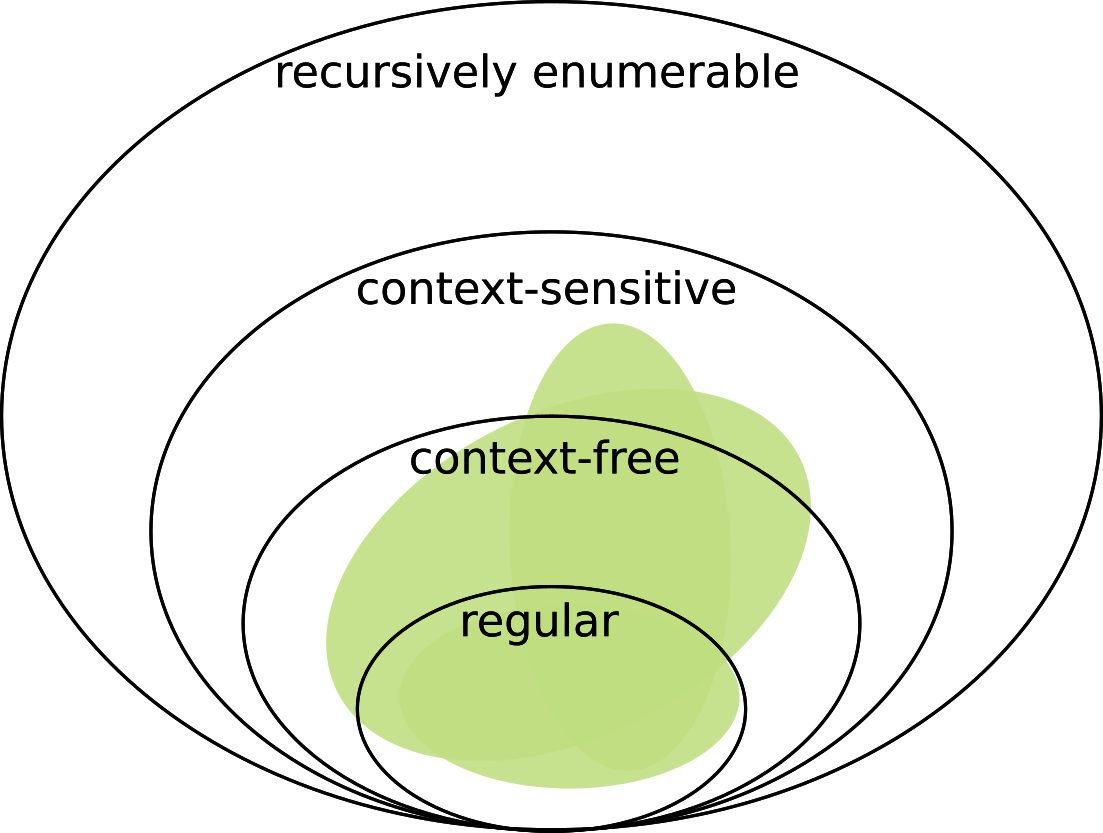
\includegraphics[width=0.4\textwidth]{chomsky.png}
  \caption{A (hypothetical) formalism that does not correspond to any single category in Chomsky hierarchy, but covers some languages in regular, some in context-free and some in context-sensitive class.}
 \label{fig:nocorr}
\end{figure}



% We start exploring the expressivity without any previous assumptions. 
% For all we know, CG may be in no particular category at all, as shown 
% in Figure~\ref{fig:nocorr}. Rather than enumerating individual grammars 
% for a given class, we need a method that can transform all languages 
% in that class into CG.

% Even if CG can express the language $a*$, it is not yet evidence 
% that whole CG is regular: for all we know, CG could just have a common subset 
% with regular languages, such as the hypothetical formalism in Figure~\ref{fig:nocorr}.

Is CG in any particular category? It clearly covers some regular languages, but 
it may just have a common subset with regular languages, such as Figure~\ref{fig:nocorr}.
Rather than enumerating individual grammars for a given class, we need a method 
that can transform all languages in that class into CG.


\section{Is CG regular?}

We present a method to transform arbitrary finite-state automata into CG.
Figure~\ref{fig:fsa} presents an example automaton, with $\Sigma = \{$\emph{det,adj,noun}$\}$,
for which we implement a corresponding CG as follows.

As a modification to \maxAmb{n}, we use \maxAmbFSA{n}:
$\Sigma$ stands for maximally ambiguous \emph{word cohorts}, and $S$ for maximally ambiguous 
\emph{state cohorts}, which are inserted between each $\langle \Sigma \rangle$.
For example, a sequence with two transitions would be modelled with the following 
sentence \maxAmbFSA{2}, with two word cohorts:

\begin{table}[h]
\centering
\begin{tabular}{lllll}
      \swf    &    \wwf      &      \swf      &     \wwf      &     \swf     \\
 ~~~~~~\t{s1} & ~~~~\t{det}  &  ~~~~\t{ s1}   &  ~~~~\t{det}  &  ~~~~\t{s1}  \\
 ~~~~~~\t{s2} & ~~~~\t{adj}  &  ~~~~\t{ s2}   &  ~~~~\t{adj}  &  ~~~~\t{s2}  \\
              & ~~~~\t{noun} &                &  ~~~~\t{noun} &  
\end{tabular}
\end{table}


The rules of the grammar disambiguate both word cohorts and state cohorts.
Thus the desired result shows both the accepted string and the path in the automaton.

\begin{table}[h]
\centering
\begin{tabular}{lllll}
      \swf    &  \wwf       &      \swf     & \wwf           & \swf \\
 ~~~~~~\t{s1} & ~~~~\t{det} &  ~~~~\t{s2}   &  ~~~~\t{noun}  &  ~~~~\t{s1} 

\end{tabular}
\end{table}



\begin{figure}[t]
  \centering
    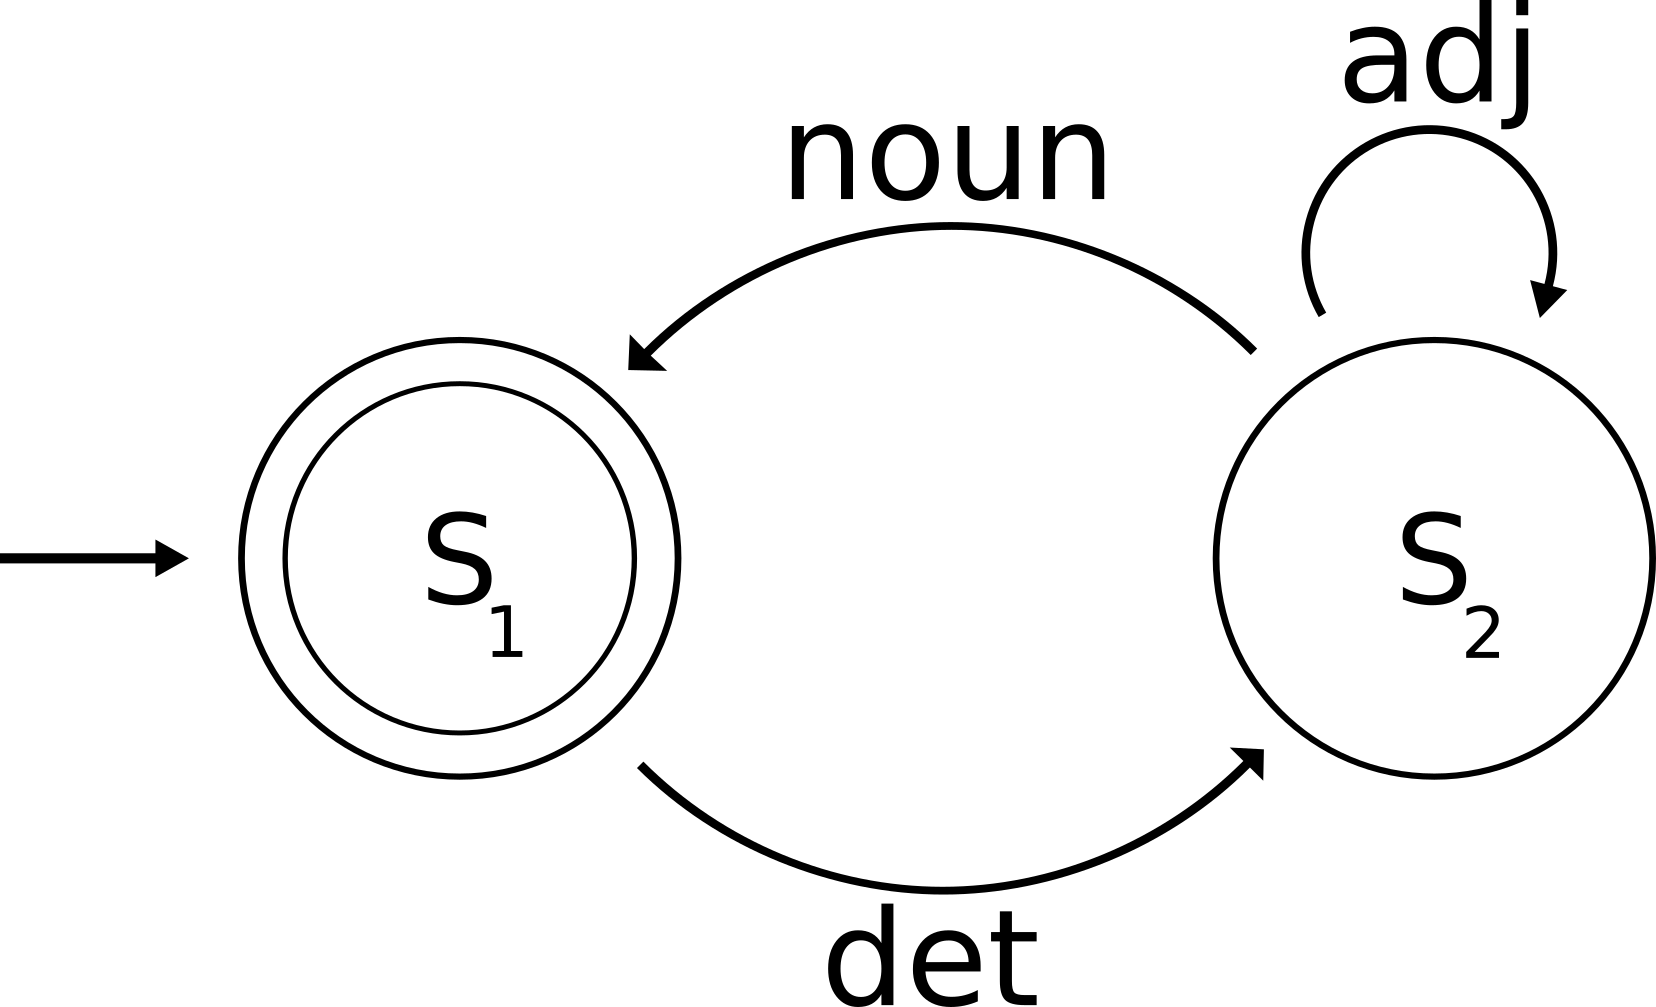
\includegraphics[width=0.3\textwidth]{fsa.png}
  \caption{A finite-state automaton describing the regular language \t{det (adj)* noun}.}
 \label{fig:fsa}
\end{figure}


\subsection{Disambiguation process}

We describe the process on a high level. We have a working implementation that
produces the rules for arbitrary automata, but the following is by no means a formal proof.

Given that every transition happens between two states, and every state 
has an incoming and outgoing transition, every rule needs no more than
positions -1 and 1 in their contextual tests. 
The semantics of the rules are ``remove a POS tag, if it is \emph{not} surrounded by allowed states'',
and ``remove a state, if it is \emph{not} surrounded by allowed transitions''.
For the example automaton, the POS-rules are as follows.

\begin{verbatim}
REMOVE...
   Det  IF (NEGATE -1 S1 LINK 2 S2) ;
   Adj  IF (NEGATE -1 S2 LINK 2 S2) ;
   Noun IF (NEGATE -1 S2 LINK 2 S1) ;
\end{verbatim}

The start and end states naturally correspond to the first and last state cohort 
in the \maxAmbFSA{n}, and can be trivially disambiguated, in this case both into \t{s1}.
Once we remove a reading from either side of a cohort, some more rules 
can take action---the context ``\t{s1} on the left side and \t{s2} on the right side''
may be broken by removing either \t{s1} or \t{s2}.
As a chain reaction, the whole sentence gets eventually disambiguated.

\subsection{Disjunction}

One obvious flaw is the lack of disjunction in CG. Consider the regular 
language with two strings $\{ab,ba\}$. Given \maxAmb{2} for any $\Sigma$,
this is the closest we could get in CG output:

\begin{table}[h]
\begin{tabular}{l l}

 \wwf          &  \wwf  \\
 ~~~~~~~~~~\t{a}  &  ~~~~~~~~~~\t{a}  \\
 ~~~~~~~~~~\t{b}  &  ~~~~~~~~~~\t{b}
\end{tabular}
\end{table}


If our alphabet consists of anything more than $\{a,b\}$, at least all the other 
readings would be removed. But CG cannot express the disjunction any further---the 
description ``either $ab$ or $ba$'' is translated into a coarser description:
 ``the first character may be either $a$ or $b$, and the second character may be either $a$ or $b$''.

Another option would be to return a set of CGs: one that disambiguates any input
into $ab$ and other that disambiguates into $ba$. But this is just speculation, 
we have not investigated the idea further. 

% The start and end states naturally correspond to the first and last state cohort 
% in the \maxAmbFSA{n}, and can be trivially disambiguated, in this case both into \t{s1}.
% The intermediate result is shown below:

% \def\rmd#1{{\tt \color{gray} #1}}

% \begin{table}[h]
% \centering
% \begin{tabular}{lllll}
%      \swf &  \wwf   &      \swf &     \wwf &     \swf \\
% ~~~~~~\t{s1}   & ~~~~\t{det}  &  ~~~~\t{s1}   &  ~~~~\t{det}  &  ~~~~\t{s1}   \\
% ~~~~~~\rmd{s2} & ~~~~\t{adj}  &  ~~~~\t{s2}   &  ~~~~\t{adj}  &  ~~~~\rmd{s2}   \\
% ~~~~~~         & ~~~~\t{noun} &                &  ~~~~\t{noun} &  
% \end{tabular}
% \end{table}

% Once we remove a reading from either side of a cohort, some more rules may take action.
% Now that the first state is no longer a possible \t{s2}, the rules that remove \t{adj}
% and \t{noun} readings will apply to the first word.

% \begin{table}[h]
% \centering
% \begin{tabular}{lllll}
%      \swf &  \wwf     &      \swf &     \wwf &     \swf \\
% ~~~~~~\t{s1}   & ~~~~\t{det}    &  ~~~~\t{ s1}   &  ~~~~\t{det}  &  ~~~~\t{s1}   \\
% ~~~~~~\rmd{s2} & ~~~~\rmd{adj}  &  ~~~~\t{ s2}   &  ~~~~\t{adj}  &  ~~~~\rmd{s2}   \\
% ~~~~~~         & ~~~~\rmd{noun} &                &  ~~~~\t{noun} &  
% \end{tabular}
% \end{table}

% Now the second state cohort can be disambiguated: transitions from \t{det} may only lead to \t{s2}, 
% so we remove \t{s1}. After that, we disambiguate the second word cohort, leaving only \t{noun}.
% No more rules may apply, so this is the final result.

% \begin{table}[h]
% \centering
% \begin{tabular}{lllll}
%       \swf &  \wwf     &      \swf &     \wwf  &     \swf \\
%  ~~~~~~\t{s1}   & ~~~~\t{det}    &  ~~~~\rmd{s1}  &  ~~~~\rmd{det} &  ~~~~\t{s1}   \\
%  ~~~~~~\rmd{s2} & ~~~~\rmd{adj}  &  ~~~~\t{s2}    &  ~~~~\rmd{adj} &  ~~~~\rmd{s2}   \\
%  ~~~~~~         & ~~~~\rmd{noun} &                &  ~~~~\t{noun}  &  
% \end{tabular}
% \end{table}





\section{Beyond regular}

We have not found a general method for other classes. 
However, we can write some example grammars that go beyond regular and context-free.

\subsection{CG is beyond regular}

We can express $a^nb^n$, here's the grammar.

\subsection{CG is beyond context-free}

We can express $a^nb^nc^n$, here's the grammar.  

\section{Applications}

Does such an idea provide any foreseeable practical benefits?
The grammars derived from FSAs look clumsy, and involve extra symbols.
But if it turned out that CGs can express some interesting subset of context-free 
or context-sensitive grammars, then we could derive CGs from already existing formalisms.
This could be an alternative for learning CGs from corpus.

Compared to high-level grammar formalisms, such as (insert your favourite), CG processing
is generally faster. So a CG derived in this manner could act as a preprocessing step 
for some more expensive parser---then the rules need not be human-legible. 
The rules would be derived from the grammar itself, with the sole purpose of 
making the parsing \emph{faster}, not more accurate.



% \section*{Acknowledgments}

% Do not number the acknowledgment section. Do not include this section
% when submitting your paper for review.





\bibliographystyle{acl}
\bibliography{cg}


\end{document}
